\section{Organizzazione aziendale}
\subsection{Aree di competenza}
{\company} è strutturata in tre aree di competenza, ognuna con ruoli e responsabilità specifiche.\\
\textbf{Reparto Assistenza}: qui operano i consulenti tecnici gestionali, il cui compito è assistere l'azienda nell'implementazione dei nuovi gestionali 
e nella gestione del cambiamento assicurandosi che il personale aziendale sia formato sull'uso delle nuove tecnologie. Ogni consulente è responsabile di uno 
o più \textit{software} di cui hanno un ampia conoscenza operativa. Inoltre, forniscono assistenza ai clienti, aiutandoli 
nella risoluzione dei problemi e, se necessario, segnalando le problematiche al reparto sviluppo che aprirà quindi un 
\textit{ticket} all'interno della piattaforma Jira (vedi capitolo \ref{chap:Tecnologie}).\\
\textbf{Area Amministrazione Commerciale e \textit{Marketing}}: In quest'area si trovano diverse competenze, tra cui:
\begin{itemize}
    \item \textbf{Responsabile \textit{marketing}}: ha il compito di realizzare strategie per promuovere l'azienda 
          e i suoi prodotti ai potenziali clienti;
    \item \textbf{Risorse umane}: ha il compito di amministrare stipendi, pensioni e \textit{benefit}, nonché di assicurarsi il rispetto da parte 
          dell'azienda delle normative sul lavoro;
    \item \textbf{Contabilità}: ha il compito di gestire e registrare le transazioni finanziarie, garantendo che tutte le attività economiche 
          siano documentate in modo accurato e trasparente;
    \item \textbf{Segreteria generale}: ha il compito di gestire e indirizzare le chiamate in entrata, gestire la posta elettronica e la 
          corrispondenza, pianificare eventi aziendali;
    \item \textbf{Segreteria commerciale}: ha il compito di mantenere le comunicazioni con i clienti fornendo informazioni su prodotti e 
          servizi e preparando offerte commerciali, contratti di vendita e documenti correlati;
    \item \textbf{Amministrazione ciclo attivo}: ha il compito di garantire una gestione efficiente delle vendite e della riscossione dei pagamenti;
    \item \textbf{Commerciale rete diretta}: ha il compito di occuparsi della vendita dei prodotti direttamente ai clienti finali;
    \item \textbf{commerciale rete indiretta}: ha il compito di gestire le vendite attraverso intermediari come distributori, rivenditori, agenti o partner commerciali;
    \item \textbf{Responsabile d'impatto}: si occupa della valutazione, pianificazione e promozione delle misure di responsabilità sociale d'impresa 
          (\gls{csr}), ovvero di tutte le iniziative attuate dall'azienda in ambito sociale e di transizione ecologica.
    \item \textbf{Amministratore} è responsabile di dirigere e gestire l'azienda nel suo complesso, assicurando che tutti i dipartimenti e le attività 
          lavorino insieme per raggiungere gli obiettivi strategici e operativi.
    \item \textbf{\textit{Product manager}} ha il compito di assicurare che i prodotti siano sviluppati in linea con le esigenze del mercato, lanciati con
          successo e gestiti efficacemente durante il loro ciclo di vita.
\end{itemize}
\textbf{Reparto Sviluppo \textit{Software}}: In quest'area troviamo:
\begin{itemize}
    \item \textbf{Sviluppatori}: possono essere \textbf{\textit{front-end}}, specializzati nello sviluppo di interfacce e della gestione dell'
          interazione uomo-macchina, \textbf{\textit{back-end}} specializzati nello sviluppo della logica del \textit{software} e nella manipolazione dei 
          dati, o \textbf{\textit{full-stack}}, in grado di operare sia come sviluppatore \textit{front-end} che \textit{back-end}.
    \item \textbf{\textit{Project manager}}: ha il compito di assicurarsi che vengano rispettati obiettivi, tempi, costi e vengano soddisfatti
          i parametri di qualità;
    \item \textbf{Direttore dello sviluppo}: ha il compito di prendere le decisioni implementative e scegliere l'architettura del \textit{software}, si 
          occupa inoltre di dirigere il team e di pianificare e assegnare i lavori da svolgere;
    \item \textbf{Analista}: si occupa di interagire con i clienti per delineare i requisiti del progetto \textit{software} e documentarli in un documento 
          di analisi.
\end{itemize}

\subsection{Metodologie di sviluppo \textit{software}}
Ho potuto notare, durante la mia esperienza di tirocinio, che gli sviluppatori utilizzano metodologie Agile per la gestione dei loro progetti.\\
Le metodologie Agile sono un'approccio alla gestione dei progetti che prevede la suddivisione del progetto 
in fasi e del lavoro in cicli brevi, al termine dei quali verranno introdotti cambiamenti che avvicinano il 
progetto sempre di più al soddisfacimento di tutti i requisiti. Questo approccio è particolarmente adattabile agli imprevisti, permettendo di reagire velocemente 
e riducendo al minimo i danni, come lo slittamento della data di completamento e conseguentemente l'aumento di denaro da destinare al progetto. 
Il manifesto Agile riporta i punti principali punti di questa filosofia:
\begin{itemize}
      \item Gli \textbf{individui e le interazioni} più che i processi e gli strumenti;
      \item Il \textbf{software funzionante} più che la documentazione esaustiva;
      \item La \textbf{collaborazione col cliente} più che la negoziazione del contratto;
      \item \textbf{Rispondere al cambiamento} più che seguire un piano.
\end{itemize}
In particolare, {\company} adotta il \textit{framework} Agile Scrum, che definisce una 
serie di principi, pratiche e cerimonie per riuscire ad assimilare nel proprio metodo di lavoro la metodologia Agile. 
Scrum richiede di suddividere il lavoro in \textit{sprint} dalla durata variabile di una fino a quattro settimane. {\company} pianifica
sprint di una settima in modo da rispondere tempestivamente a gli imprevisti ed effettuare una pianificazione più efficace.

\begin{figure}[H]
      \centering
      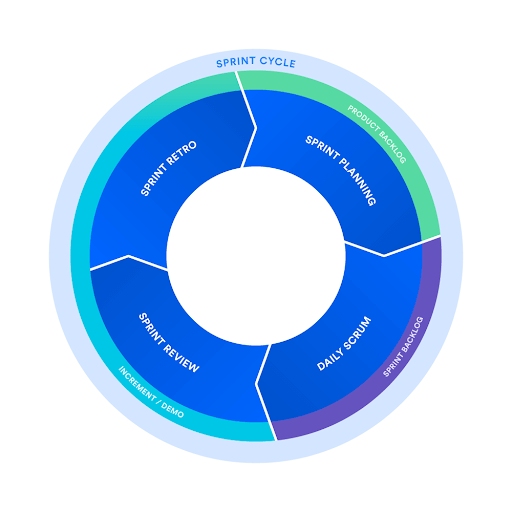
\includegraphics[alt={Organizzazione di uno sprint con il \textit{framework} Scrum}, width=0.5\textwidth]{img/scrum.png}
      \caption[Organizzazione di uno sprint con il \textit{framework} Scrum]
              {Organizzazione di uno sprint con il \textit{framework} Scrum. \\ \textit{fonte: https://www.atlassian.com/it/agile/scrum}}
      \label{fig:scrum}
  \end{figure}

Come mostrato in Figura \ref{fig:scrum} ogni sprint è strutturato in una serie di incontri che avvengono solitamente in video chiamata usando 
3CX (vedi capitolo \ref{chap:Tecnologie}).\\ 
Si comincia il lunedì, all'inizio dello \textit{sprint}, quando programmatori, direttore dello sviluppo e \textit{project manager} partecipano 
ad un \textit{meeting} chiamato \textit{sprint planning} dove si pianifica il lavoro da svolgere per lo sprint in corso.
Quindi ogni giorno si tiene un breve \textit{meeting} prima della pausa pranzo chiamato \textit{daily scrum} dove si discute dello stato dei lavori ed 
eventuali problemi emersi.
Il venerdì si tiene l'ultimo \textit{meeting} dello \textit{sprint} chiamato \textit{sprint review} dove si discute 
dello stato dei lavori rispetto alle aspettative e discutendo dei problemi emersi durante lo \textit{sprint} si cercano modi per migliorare.\\
{\company} organizza inoltre un ulteriore \textit{meeting} a cadenza mensile dove non solo le persone interessate al progetto, ma tutti i dipendenti dell'azienda 
si riuniscono per discutere dello stato dei lavori di ogni settore: \textbf{evoluzione dei prodotti, vendite, feedback dei clienti, aggiornare il reparto \textit{marketing}
 e commerciale sulle nuove funzionalità dei software ecc.}. Questo incontro ha 
lo scopo di dare a tutti i dipendenti dell'azienda una visione d'insieme evitando il cosiddetto "effetto sottomarino", ovvero quando una persona o un gruppo si focalizzano 
soltanto in uno specifico ambito, favorendo l'isolamento rispetto al resto dell'azienda, che ha invece bisogno di lavorare coordinando i vari settori.